\documentclass[a4paper]{article}

\usepackage[english]{babel}
\usepackage[utf8]{inputenc}
\usepackage{amsmath}
\DeclareMathOperator*{\argmax}{argmax}
\usepackage{graphicx}
\usepackage[colorinlistoftodos]{todonotes}

\title{Final Year Project Progress Report}

\author{Samuel Lee}

\date{16 January 2019}

\begin{document}
\maketitle

\begin{abstract}
The given data is sales data of 66 products sold over a period of 11 days without any changes in price and under some sales promotion. The objective is to use Thompson sampling to increase sales revenue in the long run and also investigate if different approaches of Thompson sampling will yield different results.
\end{abstract}

\section{Understanding the data}
\label{sec:introduction}
\begin{figure}
\centering
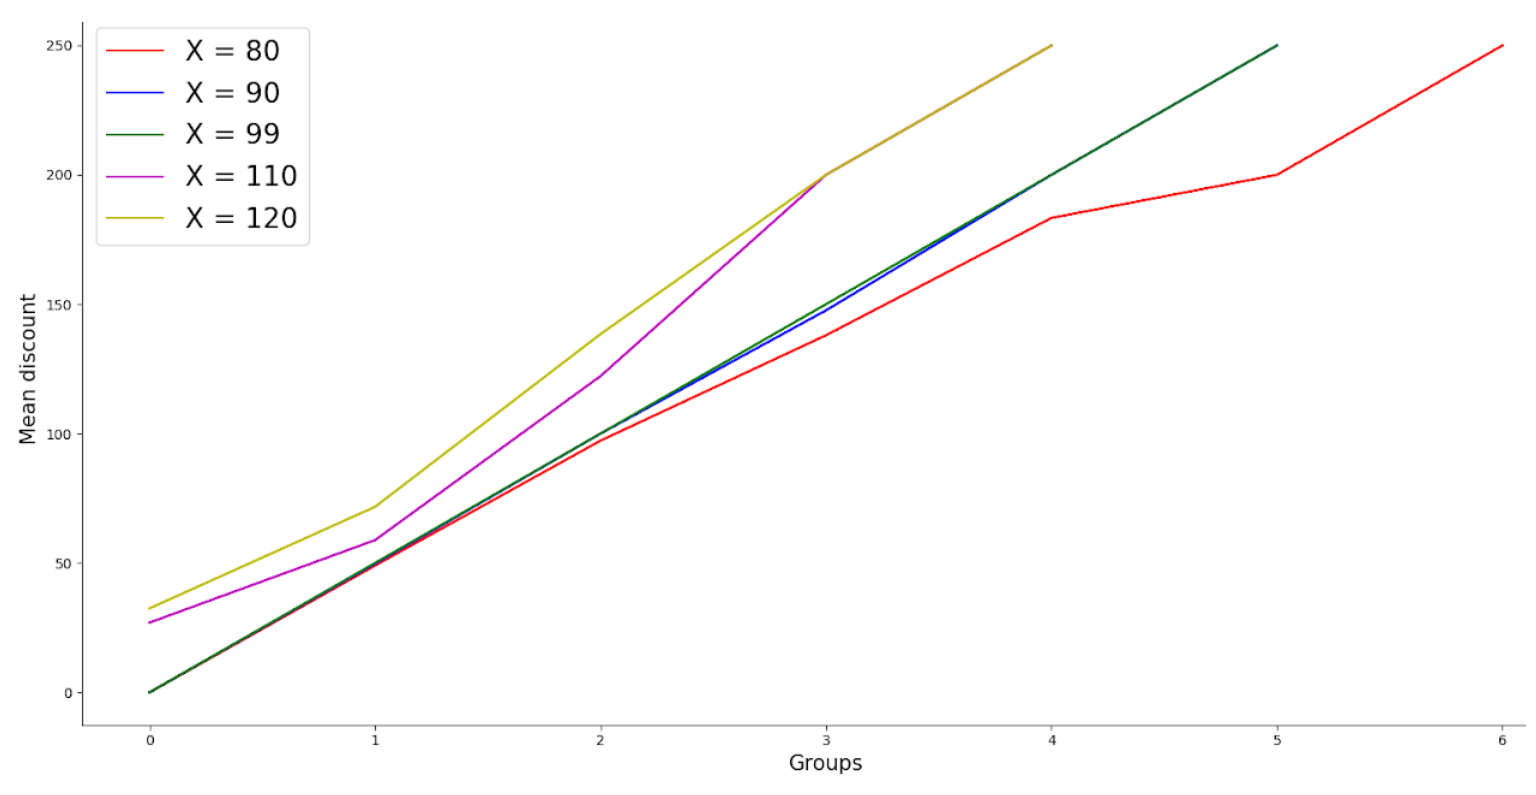
\includegraphics[width=1\textwidth]{cut.png}
\caption{\label{fig:cut}Plotting mean discounts for each group.}
\end{figure}

It is known that there is an ongoing sales promotion in the data in which an order would be eligible for discounts by fulfilling a minimum value. This value is defined as the threshold. For example, every \$99 spent would be eligible for a \$50 discount. One possible method to find the threshold would be through trial and error.
\newline
\newline
If $X$ is trialed as the threshold value, orders can be categorized into groups of different multiples of $X$. The first group would consist of orders ranging from \$0 to \$($X$-1) and the second group would range from \$$X$ to \$2$X$-1 and so on. The mean discount for each group can then be calculated. If $X$ is the threshold value, the mean discount for the first group should be 0 as all orders in that group should not have fulfilled the minimum amount. Likewise, the mean discount for subsequent groups should be multiples of the discount. Plotting the mean discounts for each group should reveal a linear relationship.
\newline
\newline
For this data set, multiple values of $X$ (80, 90, 99, 110, 120) were tested and the mean discounts were plotted. For $X = 80, 110$ and $120$, the gradients are not constant over each group. This suggests that some groups contain orders that qualify for different discounts from the rest. The plots of $X = 90$ and $X = 99$ indicate a strong linear relationship. However, at $Groups = 3$, the plot of $X = 90$ is not as linear as $X=99$. Thus, it is likely that the true threshold value of this data set is 99.

\section{Description of approaches}
\label{sec:approach}
The first approach would be to use the classical Thompson sampling algorithm in a multi-armed bandit problem where each price vector represents an arm and the objective is to investigate which arm has the highest expected payout so as to maximize revenue over time. In this approach, there is a finite number of price vectors and the goal is to learn the demand distribution of each price vector.
\newline
\newline
The second approach would be to use Thompson sampling in a dynamic pricing algorithm. In this approach, there is usually a larger set (possibly infinite) of price vectors. In this approach, the goal is to learn the distribution of the price elasticity of each product and not the distribution under each price vector.

\section{Generating training data}
\label{sec:theory}
Since the data set only contained sales data for one set of prices, there is insufficient data to perform Thompson sampling. Thus, simulation data was created and the set of prices in the data set was used as one price vector. 
\newline
\newline
For each price vector $i$, a theoretical sales data was created using the formula below and it represents the true demand under this price vector.
\[X_i = \frac{e^{V_i - P_i}}{\sum_{j=0}^{N}e^{V_j - P_j}} \tag{1}\]
where $V_i$ represents the customer's valuation of product $i$ and $P_i$ is the price of product $i$. In the denominator, $j=0$ represents the option where the customer chooses not to buy anything. For the first approach, in addition to the original price vector, two other price vectors were created where the first vector is created by adding 5 to the original price vector and the second vector is created by subtracting 5 from the original price vector. 
\newline
\newline
As there are now 3 price vectors, the valuation vector $V$ can be created by randomly sampling from a 5\% neighbourhood of $\hat{P}$ where $\hat{P}=\sum_{k=1}^{3}P_k$. $V_0$ is randomly sampled from the interval $(0,5).$
\newline
\newline
With the $V$ and $P$ vectors defined, the theoretical $X_i$ corresponding to each price vector can be created and they will represent the true demand. In the long run, the expected value of all data points for each price vector should be equal to the theoretical $X_i$.
\newline
\newline
For each price vector, 20 data points were created. In order to ensure that the expected value of all data points was equal to the theoretical $X_i$, 10 epsilon vectors were created and the data points were obtained by adding and subtracting the epsilon vector from the theoretical $X_i$. This process was repeated for the other two price vectors as well. In total, there were 60 data points created with each price vector having 20 data points.

\section{First approach}
In this approach, the objective was to learn the true demand function under each price vector. It was assumed that the true demand functions followed normal distributions. The prior distribution for each price vector was then estimated from the 20 data points generated earlier using maximum likelihood estimation. 
\newline
\newline
For iterations $k = 1,...,K$, the following process was done. 
\begin{enumerate}
	\item A random sample was taken from each price vector's prior distribution.
	\item The estimated revenue under each price vector was calculated by multiplying the random sample and the price vector since each random sample represents the estimated demand under that price vector.
	\item The price vector with the highest estimated revenue was chosen as the selected arm for this iteration.
	\item The selected arm was pulled. The observed demand would be that price vector's theoretical $X_i$.
	\item The observed revenue was calculated by multiplying the observed demand with the price vector and also accumulated over all iterations.
	\item The observed demand was added as an observation to the selected arm's $H_{k-1}$ data points where $H_{k-1}$ is the number of data points under that price vector in the previous iteration.
	\item The prior distribution of that price vector was re-estimated using the $H_{k-1} + 1$ data points.
\end{enumerate}

The number of times each price vector was selected was recorded. The price vector that was selected the most often would then be the arm with the highest revenue.
\newline
\newline
In order to validate that the chosen arm in the above process was the correct arm, a simple check was conducted for each arm. In each check, the same arm was chosen in every iteration and the observed revenue was accumulated. The arm with the greatest accumulated revenue would then be the theoretically correct arm. 
\newline
\newline
The process decribed in this approach has been able to accurately select the theoretically correct arm each time.
\section{Second approach}
In this approach, the objective was to learn the true elasticity values for each product. Since the order of prior data affects elasticity, it was assumed that the order of the price vectors implemented was as follows: lower price vector, original price vector, higher price vector. With this ordering, the prior estimates of the elasticity values could be obtained using the following formula
\[\gamma_i = \frac{\frac{x_{i,t+1}-x_{i,t}}{x_{i,t}}}{\frac{p_{i,t+1}-p_{i,t}}{p_{i,t}}}\]
where $\gamma_i$ is the elasticity of product $i$. It was assumed that the true elasticities followed a normal distribution i.e $\Pi_0(\gamma_*)=N(\mu_0,\Sigma_0)$. The prior estimates $\gamma_i$ were taken as the mean $\mu_0$ of the distribution while the covariance matrix was set as $\Sigma_0 = cI$. $c$ was set as $c = \frac{1}{10}\sum_{i=1}^{i=N}\gamma_i$
\newline
\newline
For iterations $k = 1,...,K$, the following process was done. 
\begin{enumerate}
	\item Randomly sampled from $\gamma_t \sim \Pi_{t-1}$ until all components of $\gamma_t$ are negative since elasticity values are negative.
	\item Forecasted demand $f_{i,t}$ of the following day using a vector autoregression model.
	\item Solved the following optimisation problem to get price vector $p_t$ given $p_{i,t-1}$ and estimates $f_{i,t}$ and $\gamma_t$ \[p_t = \argmax_p \sum_{i=1}^{N}\frac{p_i^2f_{i,t}\gamma_{*,i}}{p_{i,t-1}} -p_if_{i,t}\gamma_{*,i} + p_if_{i,t}\] \[\text{subject to: } p \in C_t \]
	\item Applied prices $p_t$. The observed demand would be generated by equation $(1)$ using $p_t$ and the same valuation vector $V$ in Section 3.
	\item 
	\item 
	\item 
	\item
\end{enumerate}

\section{Comparison of approaches}

\end{document}